\chapter{Diseño}
\label{ch:design}
% Explicar restricciones de tiempo, referenciar los retrasos en la planificación. Basándose en la limitación temporal, explicar la solución escogida.

Tras analizar las características tanto de Spark como de MPI, decidimos continuar la implementación haciendo uso de Spark. La herramienta de Apache tiene un mayor potencial de optimización a largo plazo y debería ser más escalable. Además, una implementaión con MPI no se alejaría demasiado de la implementación actual con Pyro.\\

Tal y como se especifica en la \autoref{sec:modificacionesCronograma}, la fase de diseño es eliminada por falta de tiempo. Sin embargo, esto no significa que pasemos directamente a la implementación de los primeros prototipos. Sigue siendo necesario especificar el diseño que se va a implementar, aunque solo sea una representación de alto nivel.\\

A partir del análisis anterior podemos realizar un diagrama de alto nivel.

\begin{figure}[H]
    \centerline{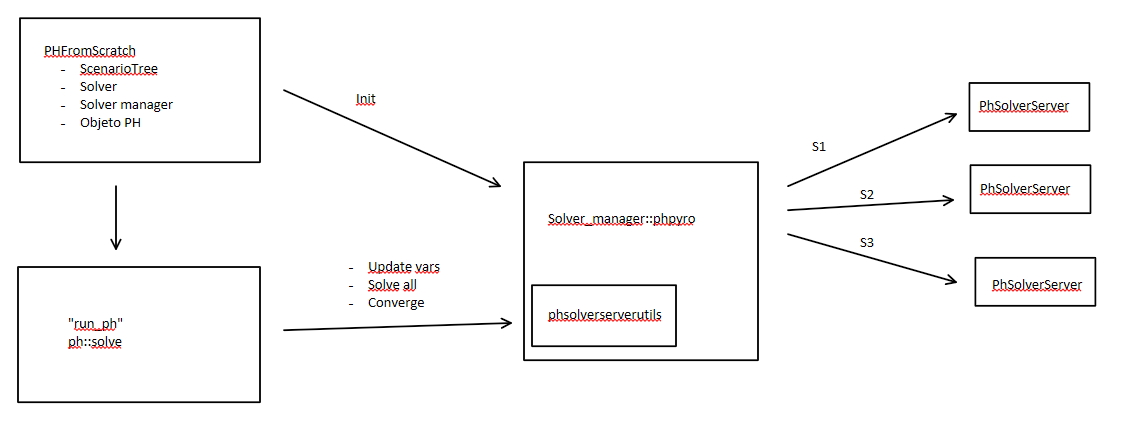
\includegraphics[width=15cm]{figuras/ph-diagram.png}}
    \caption{Diseño de runph}
    \label{fig:ph-diagram}
\end{figure}

Si tomamos el solver manager como el punto central, la parte de la derecha se ejecuta en paralelo, es decir, debemos implementarla en Spark; y la parte izquierda es la que genera los trabajos.\\

Teniendo en cuenta esta arquitectura y el tiempo disponible se propone una solución cuyo objetivo es aprovechar al máximo el código ya implementado en Pyomo y que facilite al máximo la integración de la nueva implementación. La solución propuesta es la creación de un nuevo solver manager que gestione los objetos \textit{PHSolverServer} como RDDs, donde se distribuyen los subproblemas. Con esto mantenemos el mismo sistema de ejecución mediante cola de tareas y sólo modificamos el gestor que las distribuye. 

% TODO: Intentar ampliar esto.